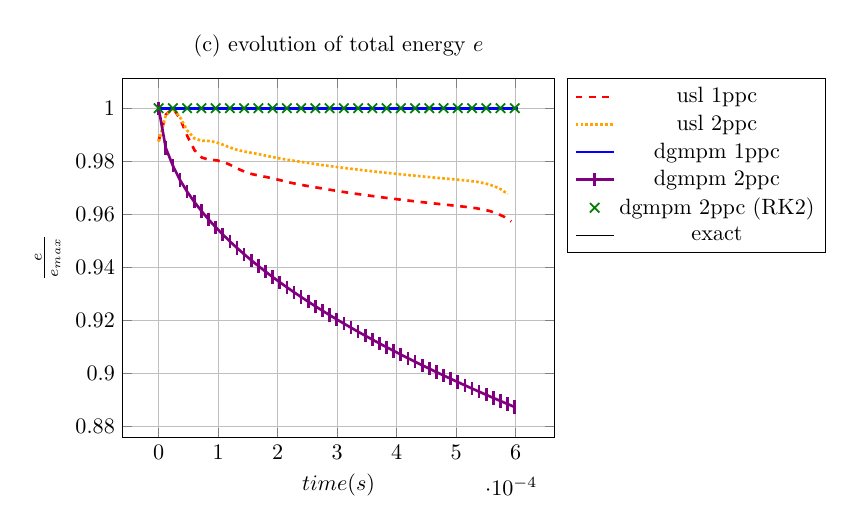
\begin{tikzpicture}[scale=0.8]
\begin{axis}[xlabel=$time (s)$,ylabel=$\frac{e}{e_{max}}$,ymajorgrids=true,xmajorgrids=true,legend pos=outer north east,title={(c) evolution of total energy $e$}]
\addplot[Red,very thick,mark=none,dashed,mark size=3pt] coordinates {(0.0,0.9876543209876545) (1.2090867953958061e-05,0.997530864197531) (2.4181735907916122e-05,1.0) (3.627260386187418e-05,0.9959104938271608) (4.8363471815832244e-05,0.9894000771604939) (6.045433976979031e-05,0.9840934847608025) (7.254520772374836e-05,0.9813625382788388) (8.463607567770642e-05,0.9805725733439128) (9.672694363166447e-05,0.9803534996362381) (0.00010881781158562253,0.9797373358436207) (0.00012090867953958059,0.97855223305006) (0.00013299954749353864,0.9771562700386213) (0.0001450904154474967,0.9759583476912668) (0.00015718128340145475,0.9751165956200767) (0.0001692721513554128,0.9745300840652308) (0.00018136301930937087,0.9740055540525709) (0.00019345388726332892,0.9734177949795755) (0.00020554475521728698,0.9727609779118863) (0.00021763562317124503,0.9721011582864625) (0.0002297264911252031,0.971500815494294) (0.00024181735907916115,0.9709763284318171) (0.0002539082270331192,0.9705033540228475) (0.0002659990949870773,0.9700475116254563) (0.00027808996294103537,0.9695899456257216) (0.00029018083089499345,0.9691327035661251) (0.00030227169884895153,0.96868819213753) (0.0003143625668029096,0.9682659231600772) (0.0003264534347568677,0.9678664411889574) (0.0003385443027108258,0.9674837019503967) (0.00035063517066478387,0.9671110350826551) (0.00036272603861874195,0.9667453037400304) (0.00037481690657270003,0.9663871533998759) (0.0003869077745266581,0.9660386728300239) (0.0003989986424806162,0.9657010208032414) (0.0004110895104345743,0.9653736208998025) (0.00042318037838853236,0.9650548630015646) (0.00043527124634249045,0.9647432582700906) (0.00044736211429644853,0.9644380781342287) (0.0004594529822504066,0.964139187671229) (0.0004715438502043647,0.9638463458344536) (0.0004836347181583228,0.9635583008484584) (0.0004957255861122808,0.9632716356128425) (0.0005078164540662388,0.9629788582366817) (0.0005199073220201969,0.9626650352466273) (0.0005319981899741549,0.9623025558244344) (0.0005440890579281129,0.9618444966372697) (0.000556179925882071,0.9612184911067746) (0.000568270793836029,0.9603246926454502) (0.000580361661789987,0.959042628998641) (0.000592452529743945,0.9572513419900455) };
\addplot[Orange,very thick,mark=none,densely dotted,mark size=3pt] coordinates {(0.0,0.9873495834618945) (1.1968737974625153e-05,0.9972230792965134) (2.3937475949250306e-05,1.0) (3.590621392387546e-05,0.996543312249306) (4.787495189850061e-05,0.9916724016989357) (5.9843689873125764e-05,0.9886458260672434) (7.181242784775092e-05,0.9877380525503068) (8.378116582237607e-05,0.9876316182265924) (9.574990379700122e-05,0.9872072095327306) (0.00010771864177162638,0.9862586211196859) (0.00011968737974625153,0.9851624959469047) (0.00013165611772087668,0.9842780087964154) (0.00014362485569550183,0.9836648835656183) (0.000155593593670127,0.9831763602119745) (0.00016756233164475214,0.9826698995825812) (0.0001795310696193773,0.9821135512367487) (0.00019149980759400245,0.9815547588976113) (0.0002034685455686276,0.9810419341151472) (0.00021543728354325275,0.9805830603182993) (0.0002274060215178779,0.9801564013202002) (0.00023937475949250306,0.9797401327914591) (0.0002513434974671282,0.979328388660163) (0.00026331223544175336,0.9789272663692082) (0.0002752809734163785,0.9785432962021172) (0.00028724971139100367,0.9781770579069166) (0.0002992184493656288,0.9778246343106916) (0.000311187187340254,0.9774820931955118) (0.0003231559253148791,0.9771479959874065) (0.0003351246632895043,0.9768228205666122) (0.00034709340126412943,0.9765071704950676) (0.0003590621392387546,0.9762007565377634) (0.00037103087721337974,0.97590260746931) (0.0003829996151880049,0.9756117726801273) (0.00039496835316263004,0.9753277223895899) (0.0004069370911372552,0.9750502574593737) (0.00041890582911188035,0.9747792209216646) (0.0004308745670865055,0.9745143288096212) (0.00044284330506113066,0.9742551920745642) (0.0004548120430357558,0.9740013948706343) (0.00046678078101038096,0.9737524481523462) (0.0004787495189850061,0.9735074554284332) (0.0004907182569596313,0.9732642558608436) (0.0005026869949342565,0.9730175918911446) (0.0005146557329088817,0.972755592971648) (0.0005266244708835069,0.9724538550537384) (0.0005385932088581321,0.9720670387858211) (0.0005505619468327574,0.971519585751107) (0.0005625306848073826,0.9706998361345011) (0.0005744994227820078,0.9694646058920318) (0.000586468160756633,0.9676621151764617) };
\addplot[Blue,very thick,mark=none,solid,mark size=3pt] coordinates {(0.0,0.9999999999999998) (2.4181735907916125e-05,0.9999999999999998) (4.836347181583225e-05,0.9999999999999998) (7.254520772374838e-05,0.9999999999999998) (9.67269436316645e-05,0.9999999999999998) (0.00012090867953958063,0.9999999999999998) (0.00014509041544749675,1.0) (0.0001692721513554129,0.9999999999999998) (0.000193453887263329,0.9999999999999998) (0.00021763562317124512,0.9999999999999998) (0.00024181735907916123,0.9999999999999998) (0.00026599909498707734,0.9999999999999997) (0.00029018083089499345,0.9999999999999997) (0.00031436256680290956,0.9999999999999997) (0.0003385443027108257,0.9999999999999997) (0.0003627260386187418,0.9999999999999997) (0.0003869077745266579,0.9999999999999997) (0.000411089510434574,0.9999999999999997) (0.0004352712463424901,0.9999999999999994) (0.00045945298225040623,0.9999999999999997) (0.00048363471815832235,0.9999999999999994) (0.0005078164540662385,0.9999999999999992) (0.0005319981899741547,0.9999999999999992) (0.0005561799258820708,0.9999999999999992) (0.000580361661789987,0.9999999999999992) (0.0006045433976979032,0.9999999999999992) };
\addplot[Purple,very thick,mark=|,solid,mark size=3pt] coordinates {(0.0,1.0) (1.1968737974625153e-05,0.9849999999999999) (2.3937475949250306e-05,0.9782812499999997) (3.590621392387546e-05,0.9728686523437499) (4.787495189850061e-05,0.9685175323486328) (5.9843689873125764e-05,0.9646764224767683) (7.181242784775092e-05,0.9612245353125033) (8.378116582237607e-05,0.9580584139595156) (9.574990379700122e-05,0.9551170218177228) (0.00010771864177162638,0.9523583400291113) (0.00011968737974625153,0.9497518470633621) (0.00013165611772087668,0.9472747764554426) (0.00014362485569550183,0.9449095127565772) (0.000155593593670127,0.942642119512832) (0.00016756233164475214,0.9404613389338139) (0.0001795310696193773,0.9383579222991295) (0.00019149980759400245,0.9363241607011475) (0.0002034685455686276,0.9343535480062032) (0.00021543728354325275,0.9324405332414724) (0.0002274060215178779,0.9305803349197901) (0.00023937475949250306,0.928768799378865) (0.0002513434974671282,0.9270022910038743) (0.00026331223544175336,0.9252776059761404) (0.0002752809734163785,0.9235919036615065) (0.00028724971139100367,0.9219426514179895) (0.0002992184493656288,0.9203275797465361) (0.000311187187340254,0.9187446455091373) (0.0003231559253148791,0.9171920015078542) (0.0003351246632895043,0.915667971129286) (0.00034709340126412943,0.914171027059833) (0.0003590621392387546,0.9126997733000616) (0.00037103087721337974,0.9112529298736883) (0.0003829996151880049,0.9098293197534216) (0.00039496835316263004,0.9084278576229242) (0.0004069370911372552,0.9070475401691336) (0.00041890582911188035,0.9056874376575983) (0.0004308745670865055,0.9043466865894064) (0.00044284330506113066,0.9030244832746345) (0.0004548120430357558,0.9017200781862146) (0.00046678078101038096,0.9004327709813899) (0.0004787495189850061,0.8991619060967203) (0.0004907182569596313,0.897906868837865) (0.0005026869949342565,0.8966670818978505) (0.0005146557329088817,0.8954420022477787) (0.0005266244708835069,0.8942311183524017) (0.0005385932088581321,0.8930339476700012) (0.0005505619468327574,0.8918500344018717) (0.0005625306848073826,0.8906789474616031) (0.0005744994227820078,0.8895202786384733) (0.000586468160756633,0.8883736409327396) (0.0005984368987312582,0.8872386670435604) };
\addplot[Green,thick,mark=x,only marks,mark size=3pt] coordinates {(0.0,1.0) (2.3937475949250306e-05,0.9999999999999997) (4.787495189850061e-05,0.9999999999999998) (7.181242784775092e-05,0.9999999999999998) (9.574990379700122e-05,0.9999999999999998) (0.00011968737974625153,0.9999999999999998) (0.00014362485569550183,0.9999999999999998) (0.00016756233164475214,0.9999999999999997) (0.00019149980759400245,0.9999999999999997) (0.00021543728354325275,0.9999999999999994) (0.00023937475949250306,0.9999999999999994) (0.00026331223544175336,0.9999999999999992) (0.00028724971139100367,0.999999999999999) (0.000311187187340254,0.999999999999999) (0.0003351246632895043,0.999999999999999) (0.0003590621392387546,0.999999999999999) (0.0003829996151880049,0.999999999999999) (0.0004069370911372552,0.999999999999999) (0.0004308745670865055,0.999999999999999) (0.0004548120430357558,0.999999999999999) (0.0004787495189850061,0.9999999999999989) (0.0005026869949342564,0.999999999999999) (0.0005266244708835067,0.999999999999999) (0.000550561946832757,0.9999999999999989) (0.0005744994227820073,0.9999999999999989) (0.0005984368987312576,0.999999999999999) };
\addplot[black,thin,mark=pentagone*,solid,mark size=3pt] coordinates {(0.0,1.0) (1e-08,1.0) };
\legend{usl 1ppc,usl 2ppc,dgmpm 1ppc,dgmpm 2ppc,dgmpm 2ppc (RK2),exact}
\end{axis}
\end{tikzpicture}
%%% Local Variables:
%%% mode: latex
%%% TeX-master: "../../mainManuscript"
%%% End:
